% Chapter Template

\chapter{Map of Profiles} % Main chapter title

\label{Chapter6} % Change X to a consecutive number; for referencing this chapter elsewhere, use \ref{ChapterX}

Load profiles can be grouped and sorted into various ways and forms.
Main attributes in order for profiles to be mapped are: 

\begin{outline}

\1 Way of metering or presenting a profile
\2 Main meter metering
\2 Appliance level metering

\1 By time range of profile 
\2 Daily
\2 Weekly
\2 Monthly
\2 Yearly

\1 Way of measuring usage
\2 Average power use 
\2 Activation or frequency of activation
\2 other (On time distribution, or on time per appliances)
\end{outline}

A most common way load profiles are presented is a daily power consumption profile such as shown on figure \ref{fig:daily_power_profile}. 
Graph is a sketch, but it represents a standard load profile with morning and evening peaks.

\begin{figure}[H]
	\centering
	\caption{"Average daily usage profile for an appliance or a building"}
	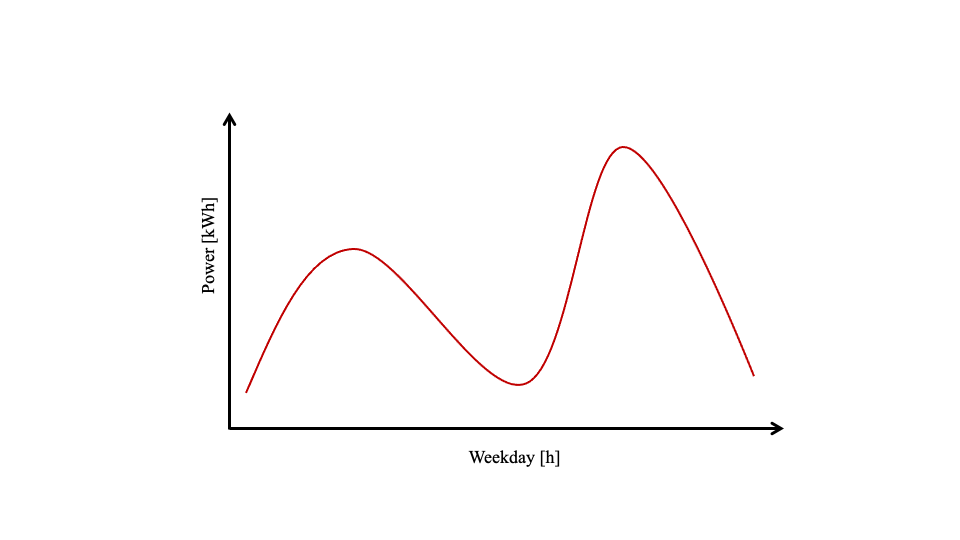
\includegraphics[width=0.9\textwidth]{Figures/profile_sketches/Slide1.png}
	\label{fig:daily_power_profile}
\end{figure}

Some refrences include daily usage profiles as a histogram of activation at a point in a day, such as figure \ref{fig:daily_act_profile}.

\begin{figure}[H]
	\centering
	\caption{"Histogram of daily activations profile for an appliance or a building"}
	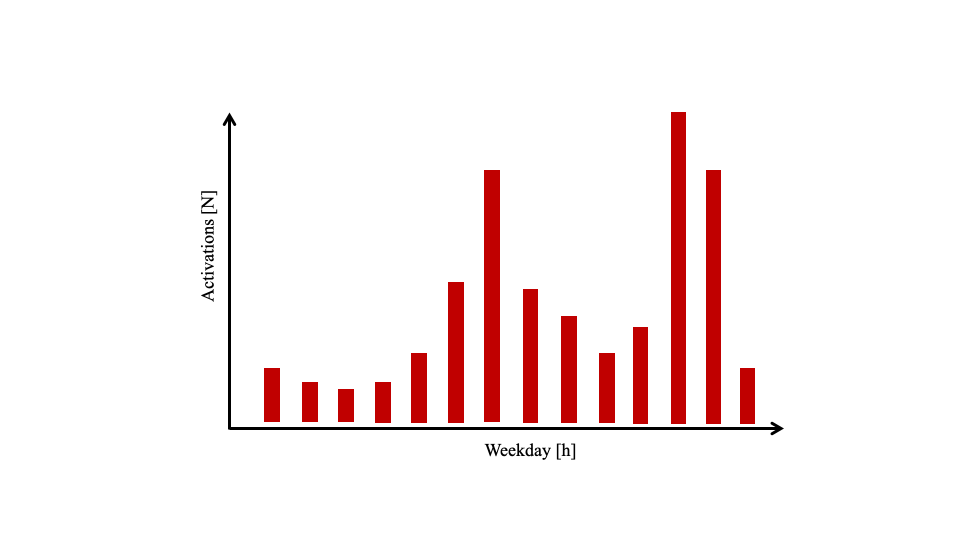
\includegraphics[width=0.9\textwidth]{Figures/profile_sketches/Slide5.png}
	\label{fig:daily_act_profile}
\end{figure}

All figures can present whole house usage or per device usage. Each representation has its pros and cons. 
To present more information sub-meter data can be used to represent whole house usage with per-appliance contributions.
Such as on figure \ref{fig:daily_act_m_profile} and \ref{fig:daily_power_m_profile}.

\begin{figure}[H]
	\centering
	\caption{"Histogram of daily activations profile for an appliance A and B"}
	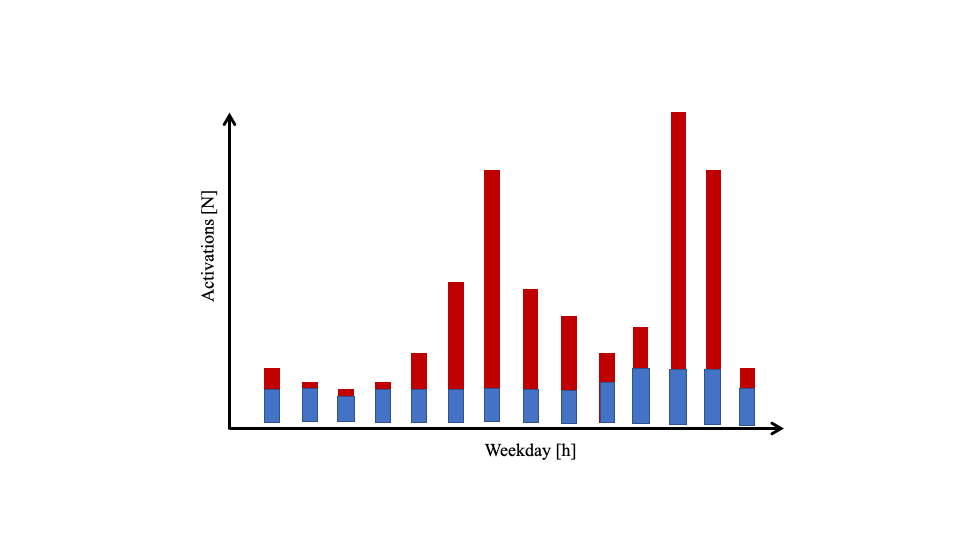
\includegraphics[width=0.9\textwidth]{Figures/profile_sketches/Slide8.png}
	\label{fig:daily_act_m_profile}
\end{figure}
\begin{figure}[H]
	\centering
	\caption{"Average weekday power consumption for appliances A, B and C"}
	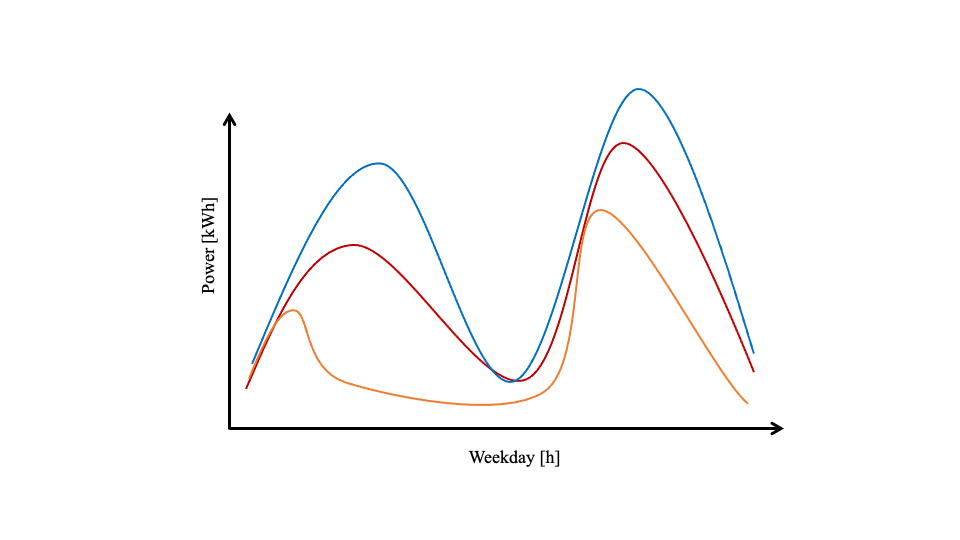
\includegraphics[width=0.9\textwidth]{Figures/profile_sketches/Slide2.png}
	\label{fig:daily_power_m_profile}
\end{figure}

To present as much information as possible all above-mentioned attributes 
can be presented in a multidimensional way such as heatmap in a way shown in figure \ref{fig:heatmap_2dtime} and \ref{fig:heatmap_all_appl}.

\begin{figure}[H]
	\centering
	\caption{"Number of daily activations / power consumption of one appliance / house in one month period"}
	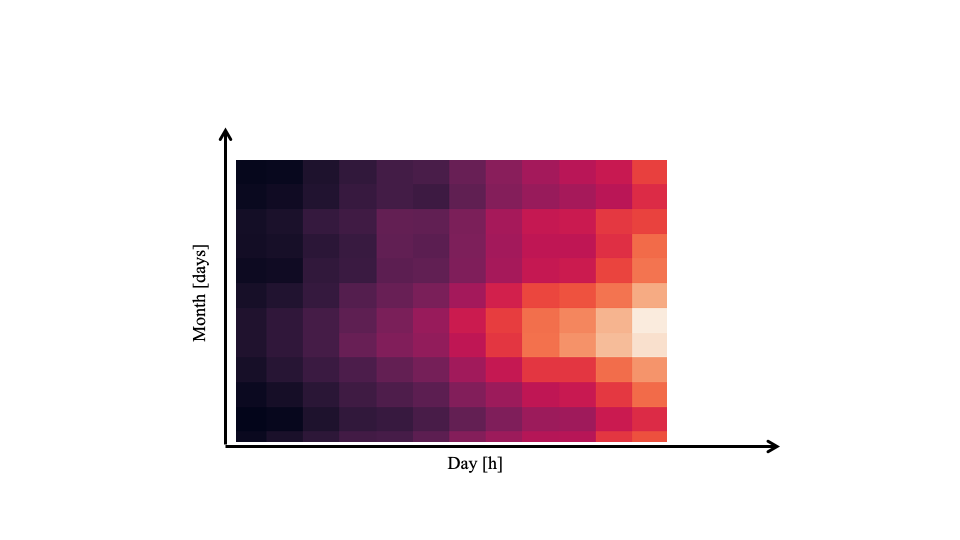
\includegraphics[width=0.9\textwidth]{Figures/profile_sketches/Slide10.png}
	\label{fig:heatmap_2dtime}
\end{figure}
\begin{figure}[H]
	\centering
	\caption{"Number of activations / power consumption for each appliance in one month period"}
	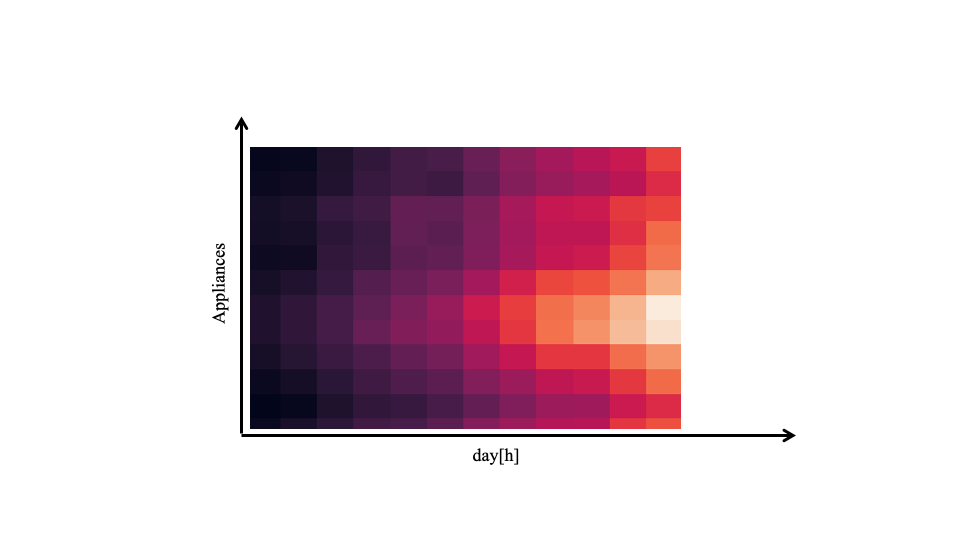
\includegraphics[width=0.9\textwidth]{Figures/profile_sketches/Slide12.png}
	\label{fig:heatmap_all_appl}
\end{figure}

Above shown profiles can be presented in combinations with each other, yielding a new way of presenting the data.
Bellow a map with combinations of above-mentioned profiles is presented. Some combinations that had similar output were grouped,
and some that were not logical were removed. 

\begin{figure}[H]
	\centering
	\caption{"Table of combinations"}
	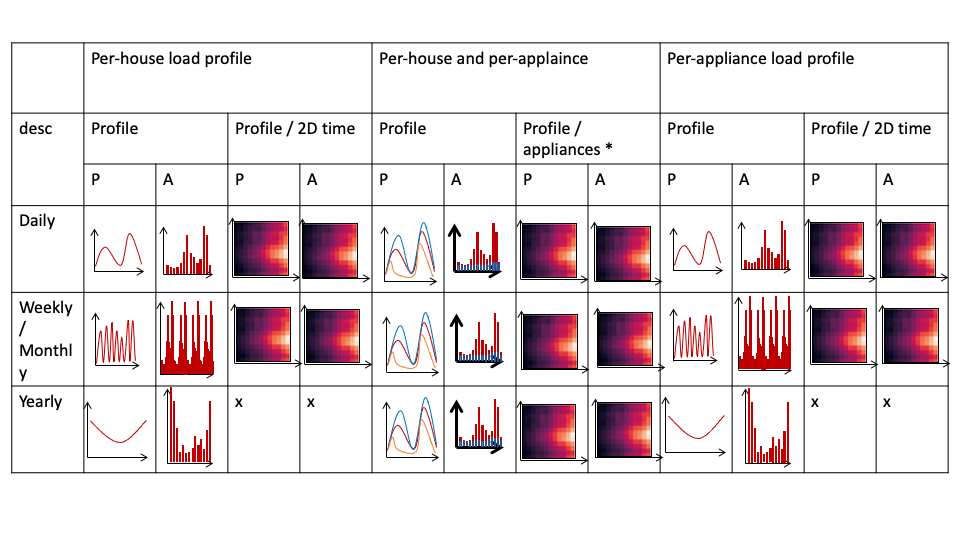
\includegraphics[width=0.9\textwidth]{Figures/profile_sketches/Slide14.png}
	\label{fig:map_fig}
\end{figure}

Table \ref{tab:contributions} shows current work done, with included refrences

testing ciytations \citeyear*{CAPASSO1994}
\begin{table}[]
	\caption{Table presents previously mentioned load profiles}
	\label{tab:contributions}

	\begin{tabular}{|l|cccc|cccc|cccc|}
	\hline
	Desription                                                   & \multicolumn{4}{c|}{Per-house}                                                                                               & \multicolumn{4}{c|}{Per-appliance}                                                                                           & \multicolumn{4}{c|}{\begin{tabular}[c]{@{}c@{}}Per-house\\ per-appliance\end{tabular}}                                                         \\
																 & \multicolumn{2}{c|}{LP}                         & \multicolumn{2}{c|}{\begin{tabular}[c]{@{}c@{}}2D \\ time LP\end{tabular}} & \multicolumn{2}{c|}{LP}                         & \multicolumn{2}{c|}{\begin{tabular}[c]{@{}c@{}}2D\\  time LP\end{tabular}} & \multicolumn{2}{c|}{LP}                               & \multicolumn{2}{c|}{\begin{tabular}[c]{@{}c@{}}Appliances\\ side by side\end{tabular}} \\ \cline{1-1}
	\begin{tabular}[c]{@{}l@{}}Range of time\\ axis\end{tabular} & \multicolumn{1}{c|}{P} & \multicolumn{1}{c|}{A} & \multicolumn{1}{c|}{P}                         & A                         & \multicolumn{1}{c|}{P} & \multicolumn{1}{c|}{A} & \multicolumn{1}{c|}{P}                         & A                         & \multicolumn{1}{c|}{P}    & \multicolumn{1}{c|}{A}    & \multicolumn{1}{c|}{P}                               & A                               \\ \hline
	Daily                                                        & \multicolumn{1}{c|}{\begin{tabular}[c]{@{}c@{}} \citeyear*{Chuan2014} \\ \citeyear*{Csoknyai2019} \\ \citeyear*{H0} \\ \citeyear*{KAVOUSIAN2013184} \\ \citeyear*{CAPASSO1994} \\ \citeyear*{WALKER1985} \\ \citeyear*{GERBEC2005} \\ \citeyear*{Gao2018} \\ \citeyear*{Jeong2021} \\ \citeyear*{Joana2012} \\ \citeyear*{DER_heatmap_profile} \end{tabular}}  & \multicolumn{1}{c|}{}  & \multicolumn{1}{c|}{\begin{tabular}[c]{@{}l@{}}  \citeyear*{Park2019} \\ \citeyear*{DER_heatmap_profile} \end{tabular}}   &    & \multicolumn{1}{c|}{\begin{tabular}[c]{@{}l@{}} \citeyear*{NILMAD2019} \\ \citeyear*{NILMAD22019} \\ \citeyear*{Issi2018} \\ \citeyear*{NILMAD2021} \\ \citeyear*{Castangia2021} \\ \citeyear*{occupancy2013}	\end{tabular}}  & \multicolumn{1}{c|}{\citeyear*{UKDALE}}  & \multicolumn{1}{c|}{}   &  \multicolumn{1}{c|}{}   & \multicolumn{1}{c|}{\begin{tabular}[c]{@{}l@{}} \citeyear*{Chuan2014} \\ \citeyear*{CAPASSO1994} \\ \citeyear*{Gao2018} 	\end{tabular}}   & \multicolumn{1}{c|}{}     & \multicolumn{1}{c|}{}      &    \\ \hline
	\begin{tabular}[c]{@{}l@{}}Weekly/\\ Monthly\end{tabular}    & \multicolumn{1}{c|}{\begin{tabular}[c]{@{}c@{}} \citeyear*{Csoknyai2019} \\ \citeyear*{H0} \\ \citeyear*{KAVOUSIAN2013184} \end{tabular}}  & \multicolumn{1}{c|}{}  & \multicolumn{1}{c|}{}                          &                           & \multicolumn{1}{c|}{}  & \multicolumn{1}{c|}{}  & \multicolumn{1}{c|}{}                          &                           & \multicolumn{1}{c|}{}     & \multicolumn{1}{c|}{}     & \multicolumn{1}{c|}{}                                &                                 \\ \hline
	Yearly                                                       & \multicolumn{1}{c|}{\begin{tabular}[c]{@{}c@{}} \citeyear*{Csoknyai2019} \\ \citeyear*{H0} \\ \citeyear*{KAVOUSIAN2013184} \end{tabular}}  & \multicolumn{1}{c|}{}  & \multicolumn{1}{c|}{}                          &                           & \multicolumn{1}{c|}{}  & \multicolumn{1}{c|}{}  & \multicolumn{1}{c|}{}                          &                           & \multicolumn{1}{c|}{}     & \multicolumn{1}{c|}{}     & \multicolumn{1}{c|}{}                                &                                 \\ \hline
	\end{tabular}
\end{table}


\begin{table}[]
	\caption{Table presents refrences mentioned in use cases chapter}
	\label{tab:use_cases}
	\begin{tabular}{|l|cccc|cccc|cccc|}
	\hline
	Desription &
	  \multicolumn{4}{c|}{Per-house} &
	  \multicolumn{4}{c|}{Per-appliance} &
	  \multicolumn{4}{c|}{\begin{tabular}[c]{@{}c@{}}Per-house\\ per-appliance\end{tabular}} \\
	 &
	  \multicolumn{2}{c|}{LP} &
	  \multicolumn{2}{c|}{\begin{tabular}[c]{@{}c@{}}2D \\ time LP\end{tabular}} &
	  \multicolumn{2}{c|}{LP} &
	  \multicolumn{2}{c|}{\begin{tabular}[c]{@{}c@{}}2D\\  time LP\end{tabular}} &
	  \multicolumn{2}{c|}{LP} &
	  \multicolumn{2}{c|}{\begin{tabular}[c]{@{}c@{}}Appliances\\ side by side\end{tabular}} \\ \cline{1-1}
	\begin{tabular}[c]{@{}l@{}}Range of time\\ axis\end{tabular} &
	  \multicolumn{1}{c|}{P} &
	  \multicolumn{1}{c|}{A} &
	  \multicolumn{1}{c|}{P} &
	  A &
	  \multicolumn{1}{c|}{P} &
	  \multicolumn{1}{c|}{A} &
	  \multicolumn{1}{c|}{P} &
	  A &
	  \multicolumn{1}{c|}{P} &
	  \multicolumn{1}{c|}{A} &
	  \multicolumn{1}{c|}{P} &
	  A \\ \hline
	Daily &
	  \multicolumn{1}{c|}{\begin{tabular}[c]{@{}c@{}} \citeyear*{energy_saving1} \\ \citeyear*{energy_saving3} \\ \citeyear*{EV2020} \\ \citeyear*{energyStealing2018} \\ \citeyear*{shift2015} \\ \citeyear*{optimiseCostShift2015} \\ \citeyear*{controll2014} \end{tabular}} &
	  \multicolumn{1}{c|}{} &
	  \multicolumn{1}{c|}{} &
	   &
	  \multicolumn{1}{c|}{\begin{tabular}[c]{@{}c@{}} \citeyear*{EV2020} \\ \citeyear*{elder1} \\ \citeyear*{elder2} \\   \citeyear*{occupancy2013}	  \end{tabular}} &
	  \multicolumn{1}{c|}{} &
	  \multicolumn{1}{c|}{} &
	   &
	  \multicolumn{1}{c|}{\citeyear*{Chuan2014}	 } &
	  \multicolumn{1}{c|}{} &
	  \multicolumn{1}{c|}{} &
	   \\ \hline
	\begin{tabular}[c]{@{}l@{}}Weekly/\\ Monthly\end{tabular} &
	  \multicolumn{1}{c|}{\begin{tabular}[c]{@{}c@{}} \citeyear*{energy_saving3} \\ \citeyear*{KAVOUSIAN2013184}  \end{tabular}} &
	  \multicolumn{1}{c|}{} &
	  \multicolumn{1}{c|}{} &
	   &
	  \multicolumn{1}{c|}{} &
	  \multicolumn{1}{c|}{} &
	  \multicolumn{1}{c|}{} &
	   &
	  \multicolumn{1}{c|}{} &
	  \multicolumn{1}{c|}{} &
	  \multicolumn{1}{c|}{} &
	   \\ \hline
	Yearly &
	  \multicolumn{1}{c|}{\begin{tabular}[c]{@{}c@{}}\citeyear*{energy_saving3}\end{tabular}} &
	  \multicolumn{1}{c|}{} &
	  \multicolumn{1}{c|}{} &
	   &
	  \multicolumn{1}{c|}{} &
	  \multicolumn{1}{c|}{} &
	  \multicolumn{1}{c|}{} &
	   &
	  \multicolumn{1}{c|}{} &
	  \multicolumn{1}{c|}{} &
	  \multicolumn{1}{c|}{} &
	   \\ \hline
	\end{tabular}
\end{table}




	\begin{table}[]
		\caption{Use case groups}
		\label{tab:groups}
		\begin{adjustbox}{width=1\textwidth}
		\begin{tabular}{|l|cccc|cccc|cccc|}
		\hline
		Description &
		  \multicolumn{4}{c|}{Per-house} &
		  \multicolumn{4}{c|}{Per-appliance} &
		  \multicolumn{4}{c|}{\begin{tabular}[c]{@{}c@{}}Per-house\\ per-appliance\end{tabular}} \\
		 &
		  \multicolumn{2}{c|}{LP} &
		  \multicolumn{2}{c|}{\begin{tabular}[c]{@{}c@{}}2D \\ time LP\end{tabular}} &
		  \multicolumn{2}{c|}{LP} &
		  \multicolumn{2}{c|}{\begin{tabular}[c]{@{}c@{}}2D\\  time LP\end{tabular}} &
		  \multicolumn{2}{c|}{LP} &
		  \multicolumn{2}{c|}{\begin{tabular}[c]{@{}c@{}}Appliances\\ side by side\end{tabular}} \\ \cline{1-1}
		\begin{tabular}[c]{@{}l@{}}Range of time\\ axis\end{tabular} &
		  \multicolumn{1}{c|}{P} &
		  \multicolumn{1}{c|}{A} &
		  \multicolumn{1}{c|}{P} &
		  A &
		  \multicolumn{1}{c|}{P} &
		  \multicolumn{1}{c|}{A} &
		  \multicolumn{1}{c|}{P} &
		  A &
		  \multicolumn{1}{c|}{P} &
		  \multicolumn{1}{c|}{A} &
		  \multicolumn{1}{c|}{P} &
		  A \\ \hline
		Daily &
		  \multicolumn{1}{c|}{\begin{tabular}[c]{@{}c@{}}energy saving \\ grid managment\\ (load shifting)\end{tabular}} &
		  \multicolumn{1}{c|}{} &
		  \multicolumn{1}{c|}{} &
		   &
		  \multicolumn{1}{c|}{\begin{tabular}[c]{@{}c@{}}anomaly detection\\ Elderly care\\ energy saving (EV)\\ occupancy\end{tabular}} &
		  \multicolumn{1}{c|}{} &
		  \multicolumn{1}{c|}{} &
		   &
		  \multicolumn{1}{c|}{\begin{tabular}[c]{@{}c@{}}grid managment\\ (load shifting)\end{tabular}} &
		  \multicolumn{1}{c|}{} &
		  \multicolumn{1}{c|}{} &
		   \\ \hline
		\begin{tabular}[c]{@{}l@{}}Weekly/\\ Monthly\end{tabular} &
		  \multicolumn{1}{c|}{energy saving} &
		  \multicolumn{1}{c|}{} &
		  \multicolumn{1}{c|}{} &
		   &
		  \multicolumn{1}{c|}{} &
		  \multicolumn{1}{c|}{} &
		  \multicolumn{1}{c|}{} &
		   &
		  \multicolumn{1}{c|}{} &
		  \multicolumn{1}{c|}{} &
		  \multicolumn{1}{c|}{} &
		   \\ \hline
		Yearly &
		  \multicolumn{1}{c|}{energy saving} &
		  \multicolumn{1}{c|}{} &
		  \multicolumn{1}{c|}{} &
		   &
		  \multicolumn{1}{c|}{} &
		  \multicolumn{1}{c|}{} &
		  \multicolumn{1}{c|}{} &
		   &
		  \multicolumn{1}{c|}{} &
		  \multicolumn{1}{c|}{} &
		  \multicolumn{1}{c|}{} &
		   \\ \hline
	\end{tabular}
	\end{adjustbox}

\end{table}